\documentclass{article}
\usepackage{multicol}
\usepackage{url}
\usepackage{graphicx}
\usepackage{enumitem}
\usepackage[margin = 1in]{geometry}
\title{Investigating Microbiome's Role in Neuropsychiatric Disorders in Quest of Novel Therapeutics Using Computational Methods.}
\author{Shakil Ahmed Rafi}
\begin{document}
\maketitle
\begin{abstract}
	The gut microbiome has been extensively and fruitfully studied using recently using machine learning tools yielding novel connections between neuropsychiatric disorders and the presence and abundance of various microbiota. However despite this recent successes the oral microbiota has received little attention in the literature let alone the machine learning treatment that the gut microbiome receives. This presents a promising research gap. The author proposes that since an emerging consensus for an oral-mirobiome-brain exists, since several robust datasets of the oral microbiome already exist, and since novel attentive transformer based models for regression, classification, and clustering of the microbiome do not exist yet, a growing and rather promising open gap exists in the literture for this to be fulfilled, and proposes this as their post-doctoral research goal.
\end{abstract}
\noindent
\begin{multicols}{2}
\section{Introduction}
The role of human host microbiomes in neuropsychiatric diseases has been studied extensively in the literature, e.g. for reviews see \cite{goswami_role_2021}, \cite{hashimoto_emerging_2023}, and \cite{bonnechere}. Furthermore they have been implicated in a number of neuropsychiatric disorders, such as ADHD, in \cite{bull-larsen_potential_2019}, in increasing severity of autism spectrum disorders, ASD, in children in \cite{TOMOVA2015179}, in Alzheimer's Disease in the elderly, in \cite{yk_microbiota-gut-brain_2018} and \cite{escobar_influence_2022}
\subsection{The gut microbiome in contrast to the oral microbiome}
Of the different microbiomes in the human body, (e.g. gut, oral, skin, vaginal), the gut microbiome is the most extensively studied in relation to neuropsychiatric disorders, see \cite{sorboni_comprehensive_2022}. It is not only the most studied but also the microbiome where modern machine learning techniques have been most frequently and fruitfully applied. 

This leaves a research gap for other microbiomes of the human body. For instance both \cite{goswami_role_2021} and \cite{tao_relationship_2024} both note the dearth of literature with respect to the oral microbiome.

\textbf{We propose, therefore, to take some of the tools, especially machine learning tools, used in gut microbiome analysis and apply them for the analysis of the oral microbiome}. We propose this for three reasons:

\begin{enumerate}[label = \roman*.]
	\item The oral microbiome is yet under-studied with the tools applied to other micribiomes, as noted earlier \cite{goswami_role_2021},\cite{tao_relationship_2024}.
	\item An emerging argument exists for an oral-microbiome-brain axis, OMBA, similar to the gut-brain axis, \cite{bowland_oral-microbiome-brain_2022}, \cite{xi_coming_2024}, \cite{y_did_2020}. The consensus seems to be that this area still needs to be studied.
	\item Large, robust, and mature datasets exist for the oral microbiomes, such as the Human Oral Microbiome Dataset, and extended Human Oral Microbiome Dataset\cite{homd}, Cultivated Oral Bacterial Genome Reference \cite{li_catalog_2023}, and even some smaller datasets such as the U.A.E. Healthy Future Study participants of 330 Emirati citizens \cite{noauthor_human_nodate}, and less specialized datasets such as FinnGen, \cite{noauthor_finngen_nodate}.
\end{enumerate}
\section{Machine Learning Methods to be Applied} 
Our main source of inspiration will be methods already applied to the gut microbiome, we will use the framework given in \cite{li_machine_2022}, and explore some of the hypotheses in \cite{tao_relationship_2024}.
\subsection{Regression and Classification via \texttt{TabNet}}
Regression in its various forms have a long history of use with predictions from microbiome, e.g. LASSO regression in using the blood microbiome to predict gut $\alpha$-diversity in \cite{wilmanski_blood_2019}. 

Indeed logistic and linear regression models have also had some use in predicting autism spectrum disorders, ASD from the oral microbiome, \cite{li_genetic_2022}. 

What the literature seems to lack is more sophisticated neural network regression and classification techniques like TabNet (introduced in \cite{arik_tabnet_2021}). Because genomic data is well-known to be large and yet quite sparse simpler regression methods may not be the best at this task. 

TabNet was introduced to tackle just this kind of problem. It uses an attention-based mechanism using a transformer-based \cite{vaswani_attention_2017} architecture where-in the model learns from a sparse but wide tabular data, extracting the salient features of the dataset as it reads the data along. It updates feature importances based on new data that it reads and assigns attention to these features updating the model. 

Attention based models have shown incredible promise in other areas of AI research such as Large Language Models (ChatGPT) and in computer vision with vision transformers and indeed continues to do so with tabular data. Indeed benchmarking with the Tabzilla Benchmarking Suite \cite{mcelfresh2023neural} shows that TabNet may out-perform traidional gradient-boosted decision trees in contexts where the dataset is extremely large with high dimensionality and where there is large sparseness in the tabular structure.

These features make advanced attention based neural networks particularly appealing for genomic analysis. Combined with the fact that the literature is already thin in the case of the oral microbiome this presents a fertile area of research. 

As an added bonus TabNet has a robust implementation in PyTorch \cite{noauthor_pytorch-tabnet_nodate} not only as a regressor but also as a classifier, making it easy to laterally transfer it from regression to classification.

We must note however the valid concern that neural network methods are thought to be less ``explainable'' compared to standard statistical methods. This is largely mitigated with TabNet, for instance \cite{MCDONNELL2023119543} notes TabNet to be interpretable and provides ``better or comparable'' results to XGBoost \& GLM with predicting insurance claims. On top of that modern tools like SHAPS \cite{lundberg_unified_2017} and LIME \cite{10.1145/2939672.2939778}, largely bridge the interpretability gap.

The author therefore proposes using TabNet, and the related TabPFN \cite{hollmann2022tabpfn} for smaller datasets as a novel way of exploring the impact of the oral microbiome in neuropsychiatric disorders.
\subsection{Clustering via Variational Autoencoders}
In a similar vein to the previous section on regression and classification we note that microbiome research, especially gut microbiome research has had a long and fruitful use of clustering algorithms for research, e.g. \cite{shi_performance_2022} looks at four such clustering techniques, k-Means, heirarchical, partition around medoids, and Dirichlet multinomial model. 

Because genomic data often has very high dimensions there has been some promising applications for variational autoencoders, VAEs, to reduce the dimensionality down and then feed the data to clustering algorithms. This technique has seen use especially in the detection of cancer e.g. \cite{hira_integrated_2021} and \cite{8983228}, and in PubMed only one example that the author can find for metagenome binning, \cite{nissen_improved_2021}.

 VAEs also have the added benefit of reducing noise, making the data smaller by discarding redundant features similar to principal component analysis (PCA) and related principal co-ordinate analysis (PoCA), making other, more traditional, analyses easier on the dataset. 
 
 Regardless, a research gap still exists in genomic analysis of the oral microbiome using variational autoencoders. This gap is even more salient considering that software tools like DeepMicro \cite{oh_deepmicro_2020}, a suite of tools for the use of variational autoencoders for genomic analysis, already exist, dramatically reducing the software overhead for such an analysis.
 
 Finally, it must be noted that the exact mechanism by which the oral microbiome affects the brain is still up for debate. Several possible mechanisms have been suggested in \cite{tao_relationship_2024}, see Figure 2. What is clear is that this mechanism could possibly be more ``direct'' in the sense that for the gut microbiome, any toxins released into the bloodstream must first be filtered by the liver before it reaches the brain whereas this is not the case for the oral microbiome \cite{tao_relationship_2024}. 
 
 This, thus means that we may expect to see stronger correlation between the presence and respective $\alpha$ and $\beta$ diversities of different microbiota and the expected predicted neuropsychiatric disorders however this is speculative, and more research on the part of the author is needed.
\section{Objective of Research}
The target of our research will be to see the impact wit
\section{Tentative Timeline and Expected Contributions and Impact}

\begin{figure*}[t]
\begin{center}
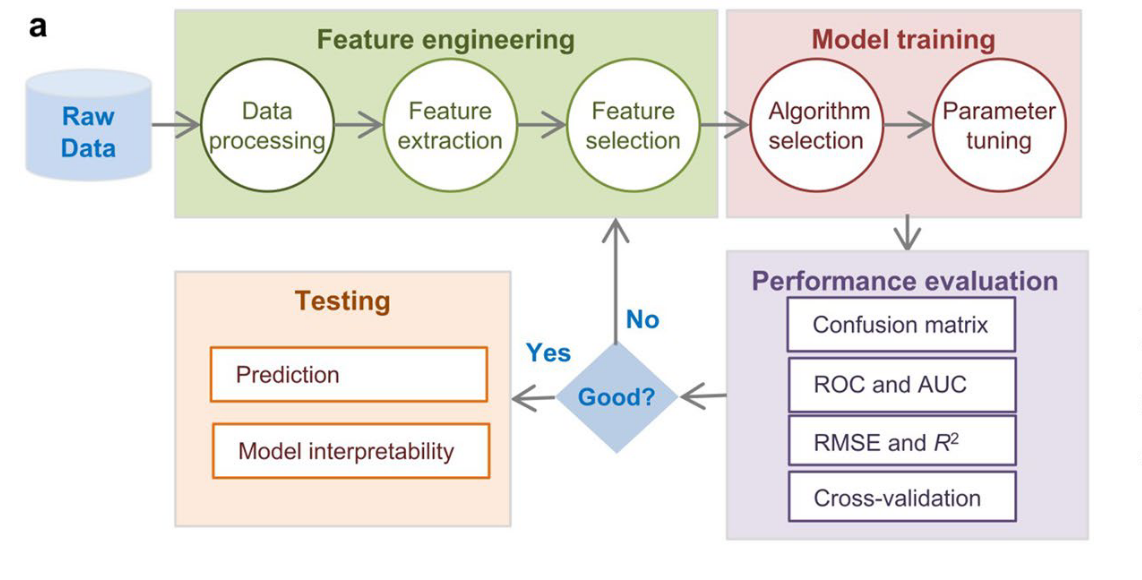
\includegraphics[width = 0.75\textwidth]{../figures/ml-workflow}
\caption{Proposed workflow for ML pipelines in genomic analysis, taken from \cite{li_machine_2022}.}
\end{center}
\end{figure*}\label{mouth}

The author proposed the following timeline for their post-doc assuming a two year period. The pipeline takes inspiration from the one proposed in \cite{li_machine_2022}, see Figure Again, this is subject to change but mostly in the direction of needing less time. 
\begin{enumerate}[label = \roman*.]
	\item Months 1-6: Explore the proposed datasets, dive deeper into the literature, and run pre-processing tasks including feature selection. This may include dimensionality reduction techniques like principal component analysis PCA, or singular value decomposition, SVM. The author also proposes to run models on a smaller subset of the data as trial runs.
	\item Months 7-12: Construct large scale models from the datasets, taking inspiration from existing literature. Steps include parameter tuning, benchmarking, and cross-validation.). 
	\item Months 13-18: Evaluate models using an appropriate metric such as RMSE, confusion matrix etc. At this stage, we may retune or reingineer features depending on the models predictive ability.
	\item Months 19-24: Dissemenate the findings in the form of papers, posters, and talks given. 
\end{enumerate}
Note that this timeline envisions a handful of models which will trained, evaluated, and retrained again, aiming for enough results to yield at-least two papers as a target.

We expect to see similar or even stronger correlations from the oral microbiome as we do with the gut microbiome, partly because of the absence of the liver mitigating whatever toxins are secreted by the oral microbiome into the bloodstream. Indeed, if it is seen that the same species in the oral microbiome is associated with the same neuropsychiatric disorder as its presence in the gut microbiome this bolsters the argument for the species as a causative agent in said neuropsychiatric disorder.


\begin{figure*}[t]
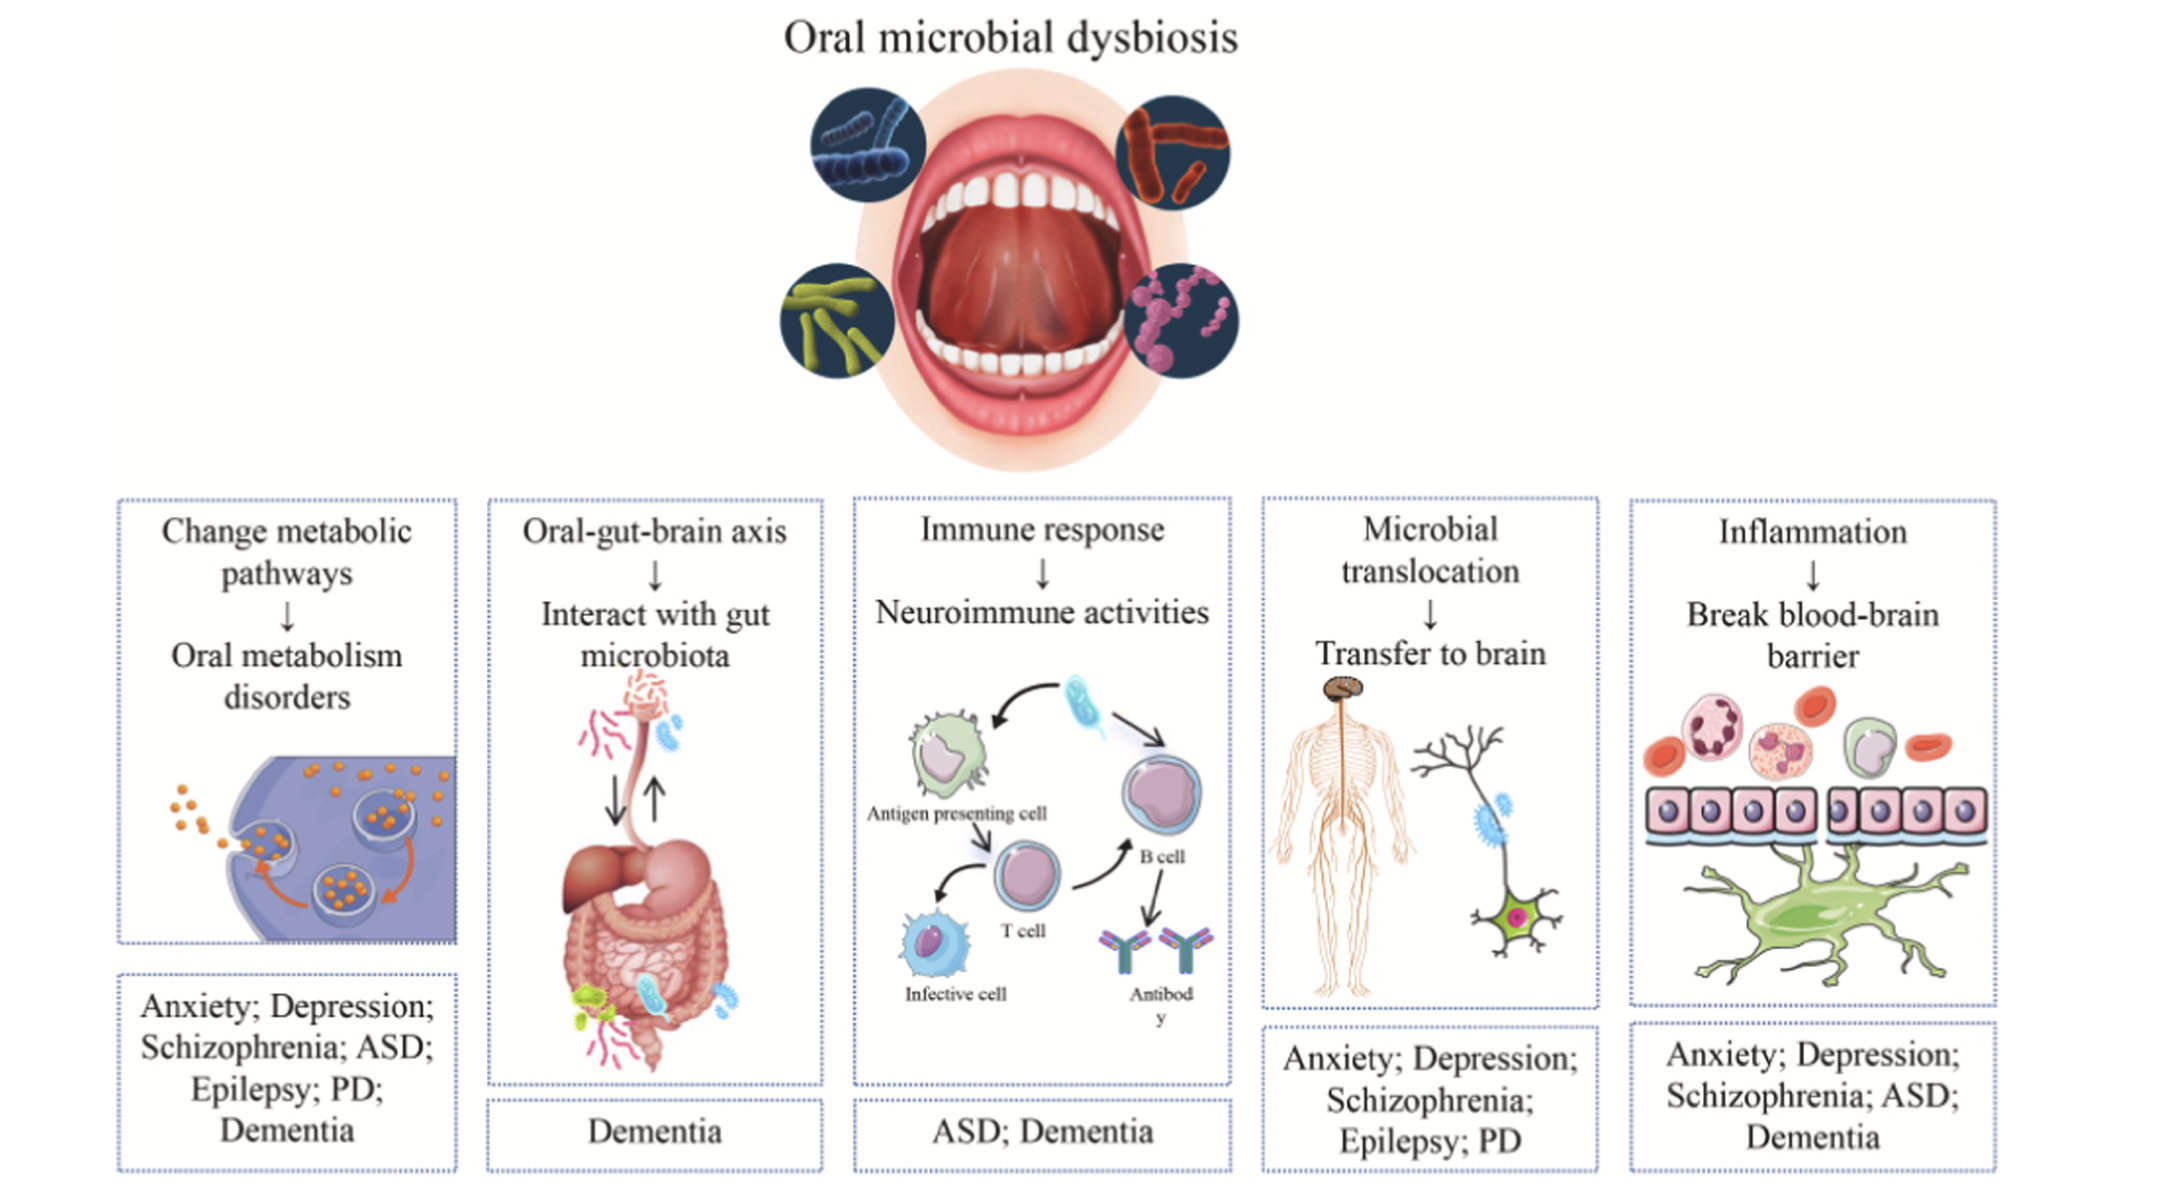
\includegraphics[width = \textwidth]{../figures/dysbiosis-oral-diagram.png}
\caption{Proposed mechanisms by which the oral microbiome may affect in neuropsychiatric disorders. Figure copied from \cite{tao_relationship_2024}, pg. 3.}
\end{figure*}\label{mouth}
\bibliographystyle{naturemag}
\bibliography{../references/goswami-proposal.bib}
\end{multicols}
\end{document}